\documentclass{article}
\usepackage{graphicx}
%\usepackage[francais]{babel}
\usepackage[utf8]{inputenc}  %% les accents dans le fichier.tex
\usepackage{lmodern}
\usepackage[T1]{fontenc}       %% Pour la cesure des mots accentues
\usepackage[paper=a4paper,textwidth=160mm,textheight=25cm]{geometry}
%\usepackage{textcomp}
\usepackage{amssymb}
\usepackage{amsmath}

\usepackage{hyperref}
\hypersetup{
    colorlinks=true,
    linkcolor=cyan,
    filecolor=magenta,
    urlcolor=blue,
}
\usepackage{xcolor}
\usepackage{listings} %% pour inclure des commandes bash
\lstset{
  frame=top,frame=bottom,
  basicstyle=\ttfamily,
  showstringspaces=false,
  commentstyle=\color{brown},
  keywordstyle=\color{red}
}
\lstdefinestyle{CStyle}{
    commentstyle=\color{brown},
    keywordstyle=\color{magenta},
    numberstyle=\tiny\color{gray},
    stringstyle=\color{blue},
    basicstyle=\footnotesize,
    breakatwhitespace=false,
    breaklines=true,
    captionpos=b,
    keepspaces=true,
    numbers=left,
    numbersep=5pt,
    showspaces=false,
    showstringspaces=false,
    showtabs=false,
    tabsize=2,
    language=C,
    morekeywords={mmg2d\_O3,Point,Circle,Line,Min,Max,Step,Name}
}


\usepackage{verbatim}
\usepackage{enumitem}
\setlist[itemize]{label=\textbullet}
\usepackage{graphicx}
\graphicspath{{./figures/}}
\usepackage{adjustbox}

\newtheorem{remark}{Remark}[section]


\newcommand{\ttb}[1]{\texttt{\textbf{#1}}}
\newcommand{\msh}{\texttt{.msh}}
\newcommand{\mesh}{\texttt{.mesh}}
\newcommand{\mmg}{\texttt{Mmg}}
\newcommand{\medit}{\texttt{Medit}}
\newcommand{\gmsh}{\texttt{Gmsh}}
\newcommand{\ra}{$\rightarrow$}


\author{Algiane Froehly}
\date{\today}
\title{Practical session: Mesh adaptation with the \mmg\ platform}

\begin{document}
\maketitle

\date{}

\section{Goals of the session:}
\begin{itemize}
\item Learn to run the \mmg\ applications;
\item Learn to call the \mmg\ libraries;
\item Understand the \mmg\ outputs;
\item Adapt a mesh to a given size map;
\item Compute an isotropic/anisotropic size map based on the interpolation error of a user-defined function.
\end{itemize}

%%%%%%%%%%%%%%%%%%%%%%%%
\section{The \mmg\ platform in short}
%%%%%%%%%%%%%%%%%%%%%%%%

The \mmg\ platform is a suite of three softwares for performing modifications on simplicial meshes (i.e. composed of triangles in 2d, tetrahedra in 3d)~:
\begin{itemize}
\item \texttt{mmg2d} is dedicated for the treatment of 2d meshes;
\item \texttt{mmgs} deals with 3d surface meshes;
\item \texttt{mmg3d} considers 3d volume meshes.
\end{itemize}
These three softwares perform quite similar operations in their respective settings:  
quality improvement of a user-supplied mesh, mesh adaptation to a size
map (isotropic/anisotropic) and level set discretization.\\

A more exhaustive documentation of the \mmg\ softwares may be founded at the following addresses:
\begin{center}
\url{http://www.mmgtools.org/mmg-remesher-try-mmg/mmg-remesher-tutorials} ,  
\end{center}
and 
\begin{center}
\url{http://www.mmgtools.org/mmg-remesher-try-mmg/mmg-remesher-options} . 
\end{center}

%%%%%%
\subsection{Installation of \mmg}
%%%%%%%
\begin{enumerate}
\item Clone the \mmg\ repository and build the applications, libraries and Doxygen documentation:
  \begin{lstlisting}[language=bash,breaklines=true,breakindent=0pt,columns=fullflexible]
    $ git clone https://github.com/MmgTools/mmg.git
    $ cd mmg
    $ mkdir build
    $ cd build
    $ cmake ..
    $ make
    $ make doc
  \end{lstlisting}
\item if your are root, you may use the \texttt{make install} command too.
\item otherwise, add the path of the \ttb{build/bin} folder to your \ttb{PATH}
  variable to be able to run the applications from your terminal
  without adding the full binary path \begin{lstlisting}[language=bash]
  $ echo "PATH=$PATH_TO_BIN:$PATH" >> ~/.bashrc
  $ source ~/.bashrc
\end{lstlisting}
In the above command line, \ttb{\$PATH\_TO\_BIN} has to be replaced by your path through the \mmg \ttb{build/bin} directory.

\end{enumerate}

\subsection{Mesh vizualisation}
You can choose to save your meshes either at the native \mmg\ file format (\mesh) and then
to vizualize your mesh with the \medit\ software (advised) or as a \gmsh\ file
format (\msh), in which case you must use \gmsh\ to vizualize your mesh.

\subsubsection{Medit installation}
\medit\ is an OpenGL-based scientific visualization software that can be downloaded on Github:
\begin{center}
\url{https://github.com/ISCDtoolbox/Medit}.
\end{center}
 A documentation (in French) is available at:
 \begin{center}
\url{https://www.ljll.math.upmc.fr/frey/logiciels/Docmedit.dir/index.html}.
\end{center}

To build \medit\, you need to have git and CMake on your PC. Then:
\begin{lstlisting}[language=bash]
$ git clone https://github.com/ISCDtoolbox/Medit.git
$ cd Medit
$ mkdir build
$ cd build
$ cmake ..
$ make
$ make install
\end{lstlisting}
\medit\ is automatically installed in the folder \ttb{\textasciitilde/bin}, and you can add this path to your \ttb{PATH}
  variable:
\begin{lstlisting}[language=bash]
  $ echo "PATH=~/bin:$PATH" >> ~/.bashrc
  $ source ~/.bashrc

\end{lstlisting}

\paragraph{Graphic packages for linux}
\begin{itemize}
\item GLUT: \tt{apt-get install -y freeglut3-dev}
\item GLUT-Xi: \tt{apt-get install -y libxi-dev}
\item GLUT-Xmu: \tt{apt-get install -y libxmu-dev}
\end{itemize}


\subsubsection{Medit main commands}
To try out \medit, you can use the \ttb{linkrods.mesh} file provided in the \ttb{TP/Data} directory of this repository. To vizualize your mesh, simply run:
\begin{lstlisting}[language=bash]
$ medit $MESH_PATH/linkrods.mesh
\end{lstlisting}
where \ttb{\$MESH\_PATH} is the path toward the \ttb{TP/Data} folder. 

\medit\ prints some mesh statistics in your terminal among which:
\begin{itemize}
\item The number of each entity in the mesh (vertices, triangles...);
\item The size of the mesh bounding box;
\item If a solution file (\ttb{.sol}) file as been read.\\
\end{itemize}


You can click on the graphic window and:
\begin{itemize}
\item Rotate the object by maintaining \ttb{left click} and moving the mouse;
\item Translate it with \ttb{alt+left click};
\item Zoom with the \ttb{z} key and unzoom with \ttb{Z};
\item Print/remove the mesh lines with \ttb{l};
\item Print colors by clicking on \ttb{c};
\item Print colors associated to the entities reference with \ttb{e};
\item Print the mesh singularities with \ttb{g}. Required points
  appears in green, corners and ridges in red and edges in different colors
  depending on their references (orange for a 0 ref);
\item Inspect the inside mesh (\ttb{clipping mode}, 3D only):
\begin{itemize}
\item Cut/uncut the mesh along a plane with \ttb{F1};
\item Edit/unedit this plane (\ttb{F2}) and rotate it (\ttb{left click}) or translate it (\ttb{alt+left click});
\item Print/unprint volume mesh with \ttb{F4};
\end{itemize}
\item Delete (resp. undelete) elements of a given color:
  \ttb{shift-click} on one element of this color, then press \ttb{r} (resp. \ttb{R});
\item Quit \medit\ with \ttb{q}.
\end{itemize}

\section{Getting started with the remeshing mode of \mmg}
To run the remesher, you simply have to enter the name of the program (by default \texttt{mmg2d\_O3} for a 2d remeshing), 
followed by the path and mesh name. 
For instance, remeshing the 2d mesh \ttb{naca\_embedded.mesh} mesh
provided in the \ttb{TP/Data} directory of this repository is achieved by the following command line:

\begin{lstlisting}[language=bash]
$ cd TP
$ mmg2d_O3 Data/naca_embedded.mesh
\end{lstlisting}

By default, the output mesh lies in the same path and has the same
extension as the input mesh (\ttb{.mesh} here) with the \ttb{.o}
prefix before the extension; in the above case: \ttb{Data/naca\_embedded.o.mesh}.

\subsection{Getting help}

You can get help by using the \ttb{-h} argument in the command line:
\begin{lstlisting}[language=bash]
$ mmg2d_O3 -h
\end{lstlisting}
%
Man pages are available in the \ttb{doc/man} directory:
\begin{lstlisting}[language=bash]
$ man ../doc/man/mmg2d.1.gz
\end{lstlisting}

If successfully builded, Doxygen documentation can be opened in the folder
\begin{center}
\ttb{build/doc/\$EXEC\_NAME/html/index.html} 
\end{center}
where
\ttb{EXEC\_NAME} stands for \texttt{mmg2d},\texttt{mmg3d} or \texttt{mmgs} depending on the context. 

You may alternatively open this help file in your
web browser by supplying the address 
\begin{center} 
\ttb{file:///\$PATH\_TO\_BUILD/build/doc/\$EXEC\_NAME/html/index.html},
\end{center}
where \ttb{\$PATH\_TO\_BUILD} has to be replaced by your path through
the \mmg\ build directory.

\subsection{The output of \mmg\ runs}
The output of the computation is displayed in the terminal; see figure \ref{mmg_konsole} for an example. 
By default, \mmg\ prints:
\begin{itemize}
\item The different phases of the algorithm (analysis step, remeshing
  step...) and the time spent in each of them;
\item Some info about the input/output element qualities;
\item The final mesh statistics (number of nodes, elements and edges).
\end{itemize}
\begin{figure}
\centering
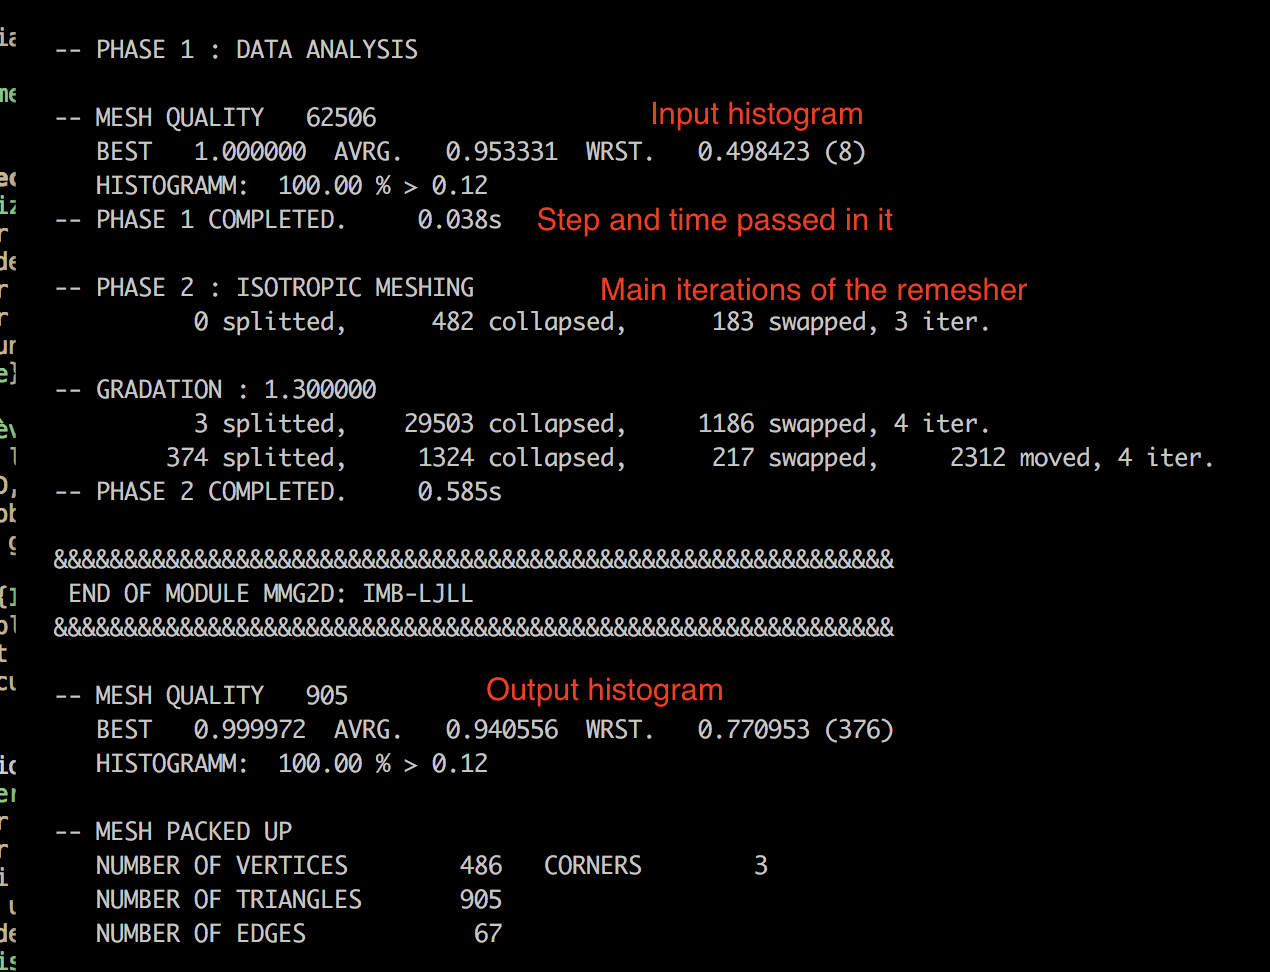
\includegraphics[width=0.8\linewidth]{mmg_konsole}
\caption{\label{mmg_konsole}
A typical default \mmg\ output.}
\end{figure}

You may change the default verbosity of \mmg\ with the \ttb{-v}
option. By default, the verbosity value is 1. For instance, turning this verbosity to 5 by using 
\begin{center}
\ttb{ mmg2d\_O3 Data/naca\_embedded.mesh -v 5},
\end{center} 
allows to display:
\begin{itemize}
\item Detailed quality histograms (see figure \ref{qual_histo});
\item Detailed remeshing steps;
\item Edge length histogram (see figure \ref{edge_histo}).
\end{itemize}

\begin{figure}
\centering
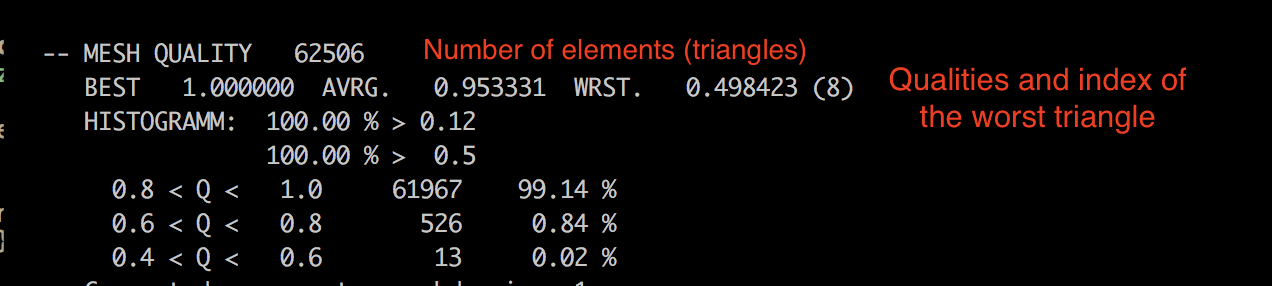
\includegraphics[width=0.8\linewidth]{qual_histo}
\caption{\label{qual_histo}
A detailed quality histogram.}
\end{figure}

\begin{figure}
\centering
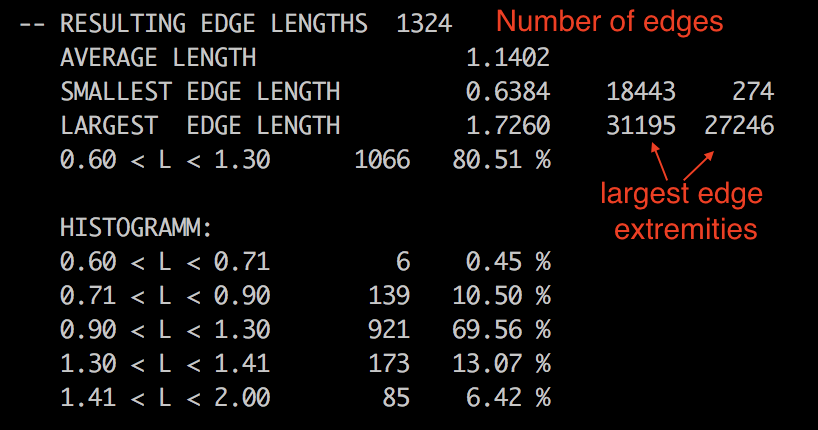
\includegraphics[width=0.8\linewidth]{edge_histo}
\caption{\label{edge_histo}
An edge length histogram.}
\end{figure}

\subsection{The four main parameters of \mmg}
By default, \mmg\ creates a mesh
that complies with 
\begin{itemize}
\item The minimum length of an edge in the mesh, controlled by the \ttb{-hmin} command line parameter; 
\item The maximum length of an edge in the mesh, controlled by the \ttb{-hmax} command line parameter; 
\item The required boundary approximation, controlled by the \ttb{-hausd} parameter; see Section \ref{sec.hausd} below about this point; 
\item the maximal ratio between two adjacent edges, controlled by the \ttb{-hgrad} parameter: the ration between the length of two adjacent edges $e_1$, $e_2$ in the mesh satisfies
$$ \frac{1}{\ttb{hgrad}} \leq \frac{| e_1|}{| e_2|} \leq \ttb{hgrad}; $$
this parameter is set to 1.3 by default. 
\end{itemize} 

\subsection{Mesh improvement with edge length preservation: -optim option}

\textcolor{red}{Pas tr\`es clair ce que tu entends par l\`a : veux-tu dire que tu gardes les m\^emes longueurs dans une r\'egion donn\'ee... ?}
 If you wish to preserve the edge length of the input mesh, you can run Mmg with
the \ttb{-optim} option~:
\begin{lstlisting}[language=bash]
$ mmg2d_O3 Data/naca_embedded.mesh -optim -v 5
\end{lstlisting}
Compare the input and output quality/lengths histograms and check that
your ouput mesh is of the same size than the input one.\\

Open the input and output meshes \ttb{medit Data/naca\_embedded.mesh} and 
  \ttb{Data/naca\_embedded.o.mesh}, and check that the edge lengths are
preserved. 

You can visualize the metric computed by \mmg\ according to the edge length in the input mesh (see Section \ref{sec.meshsizemap} to get a hint of how \mmg\ uses this information to proceed to remeshing). 
To this end, using \medit, select the window associated to the output mesh and press \ttb{m} (you may need to
remove the mesh lines with \ttb{l}).\\

If you want, you can play with other \mmg\ options~: you may for instance try
to run \mmg\ without the \ttb{-optim} option and to disable the gradation
(\ttb{-hgrad -1}).

\subsection{Boundary approximation}\label{sec.hausd}
In order to better approach the naca geometry, it is desirable to adapt the mesh to the curvature of the boundary - i.e. to impose smaller elements where the boundary of the naca is more curved.
To this end,
\begin{enumerate}
\item Look at the size of the naca airfoil (in \medit, zoom over the
naca and select a vertex near the top of the naca (alt+shift+left
click) and another near the bottom. The point coordinates are printed
in the terminal so you can evaluate the naca thickness);
\item Try a hausdorff value related to this length and decrease the minimal edge
size in consequence (for example \ttb{-hausd 0.0001 -hmin 0.000001})
\end{enumerate}

\textbf{\\Why do I need to specify \ttb{hmin} in addition to the hausdorff parameter?\\}
To avoid numerical errors (notably division by 0) and users mistakes (0 length
edges asked), \mmg\ automatically computes a minimal edge size. If a
size map is provided (see Section \ref{sec.meshsizemap}), this minimal edge size is smallest than the
smallest required length but if the user does not supply a size map, a length information is extracted from the initial mesh: in this case,
by default, \mmg\ sets \ttb{hmin} to 0.1 times the mesh bounding box
size. In our case, because the naca is a very small object in an
infinite box, the default \ttb{hmin} value is too large when a finer boundary approximation is desired.

\subsection{3d boundary approximation}
In this subsection, we will use the \ttb{thinker.mesh} mesh provided
in the \ttb{Data} folder. It is a 3d surface mesh so
\ttb{mmgs} is used in order to remesh it.

\begin{remark}
The input mesh is a non conforming mesh (see under the
bed plate). \mmg\ does not detect such patterns and is not supposed to work on it.
In the \ttb{thinker} case, it just leads to a warning:\\
\ttb{\#\# Warning: anaelt: flattened angle around ridge. Unable to split it.\\}
 and the approximation of the non conforming area is pretty bad.
 \end{remark}

\textcolor{red}{On n'a pas une version conforme du thinker ?}

\subsubsection{Mesh analysis without any modification}
\mmg\ allows to choose the remeshing operators that are applied. By
default, insertion/collapse, edge swapping and vertex relocation are
authorized. You can manually disabled each one of this operator:
\begin{itemize}
\item No point insertion/collapse: \ttb{-noinsert} command line argument;
\item No edge swapping: \ttb{-noswap};
\item No point relocation: \ttb{-nomove}.
\end{itemize}

If you combine these 3 options, \mmg\ does not modify the input mesh but only
performs the analysis. Thus, the output mesh contains the singularities
detected by the remesher on the initial mesh. This combination can
also be used to convert a \gmsh\ file into a \mmg\ one or vice versa.

\subsubsection{Edge detection}
\begin{enumerate}
\item Analyze your mesh with the default edge detection value. Use
  \medit\ to vizualize the detected singularities.
\item Increase/decrease this value (\ttb{-ar \textit{val}}) to see the
  effect on the sharp angle (ridge) detection (analysis only);
\item Analyze your mesh without the detection of sharp angle( \ttb{-nr} option).
You can see that there remain very few ridges. The only remaining ones are:
\begin{itemize}
\item Non-manifold edges: edges at the intersection of a surface and
  a hanging surface (so the surfaces intersect in a T-shaped pattern);
\item The boundary edges of an open surface.
\end{itemize}
\item Remesh your mesh with a suitable value for the ridge detection angle.
\end{enumerate}

\subsubsection{Play with the hausdorff parameter}
\begin{enumerate}
\item Open your mesh with \medit\ to get the size of its bounding box;
\item Evaluate the order of amplitude for the Hausdorff parameter;
\item Try out several values of the hausdorff parameter (\ttb{-hausd} \textit{val}).
\end{enumerate}

\section{Mesh adaptation to a size map}\label{sec.meshsizemap}
It is possible to supply \mmg\ with a size map in a \ttb{.sol} file. The role of this file
is to prescribe a desired local edge length around each vertex in the mesh. 

\begin{itemize}
\item In the case of \textit{isotropic} mesh adaptation,
1 scalar data is supplied per node (the wanted edge length around it). 
\item In the case of \textit{anisotropic} mesh adaptation, this file supplies a metric tensor $M$ at each vertex, that can be
diagonalized in the eigenbasis:
$$
M = R\, \Lambda \, R^{-1} , 
$$
where:
\begin{itemize}
\item $R = (r_{ij})_{ij}$ is the matrix of the eigenvectors;
\item $\Lambda = (\lambda_j)_j$ is the diagonal matrix containing the eigenvalues of $M$.
\end{itemize}
A given eigenvalue $\lambda_j$ and the
desired edge length $s_j$ in the direction of this the eigenvector $r_j$ are related as: 
$$\lambda_j=\frac{1}{s_j^2}.$$
\end{itemize} 

See Figure \ref{map} for an explanation of the \ttb{.sol} file format
for both isotropic and anisotropic size maps.\\

\begin{figure}
\centering
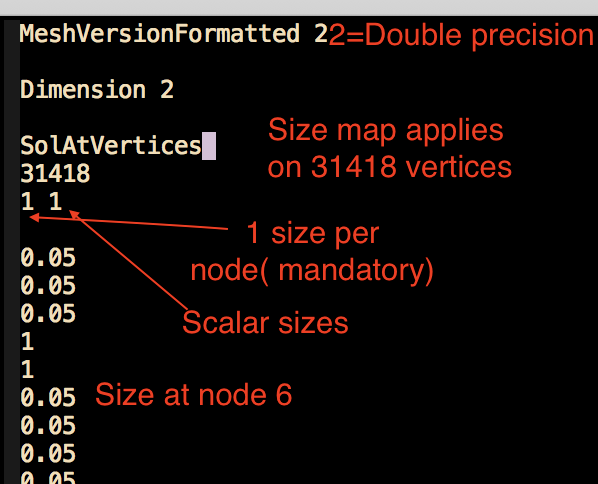
\includegraphics[width=0.4\linewidth]{iso_map}
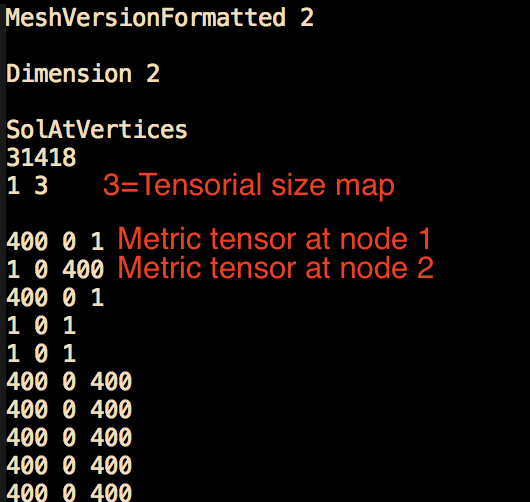
\includegraphics[width=0.4\linewidth]{aniso_map}
\caption{\label{map}
Isotropic (left) and anisotropic (right) size maps at \ttb{medit} file format.}
\end{figure}

\begin{figure}
\centering

\end{figure}


You will find in the \ttb{Data} directory two size maps (\ttb{naca\_iso.sol} and
\ttb{naca\_aniso.sol}) for the
\ttb{naca\_embedded.mesh} 2D mesh. A adapt your mesh to each map. For
example, for the isotropic map~:
\begin{lstlisting}[language=bash]
$ mmg2d_O3 Data/naca_embedded.mesh -sol naca_iso.sol -hausd 0.001 -v 5
\end{lstlisting}

Again, you may play with the gradation parameter \ttb{-hgrad}.

%%%%%%%%%%%%%%%%%%%%%%%%%%%%%%%%
\section{Calling the \mmg\ libraries to manually compute a size map\label{size_map}}
%%%%%%%%%%%%%%%%%%%%%%%%%%%%%%%%
The \mmg\ library may be called from \ttb{C}, \ttb{C++} or \ttb{Fortran} codes by
using its API functions.\\
\\
In this section, we shall create a size map for the
\ttb{naca\_embeddded.mesh} mesh and call the Mmg library.

 You can
start either from the \ttb{Data/firstSizeMap.c} or
\ttb{Data/firstSizeMap.F90} file.\\
Now, follow the program:
\begin{enumerate}
\item Include the \ttb{mmg2d} header file (needed to know the \mmg\ structures):
\begin{center}
\ttb{\#include "mmg/mmg2d/libmmg2df.h".}
\end{center}
\item Initialize the \mmg\ structures (\ttb{MMG2D\_Init\_mesh} function);
\item Load the mesh (\ttb{MMG2D\_loadMesh} function);
\item Save the initial mesh and metric in the \ttb{init.mesh} and
  \ttb{init.sol} files (\ttb{MMG2D\_saveMesh} and \ttb{MMG2D\_saveSol}
  functions). Note that if the solution has not been set, it is not saved.
\item Set the hausdorff parameter to 0.0001 (\ttb{MMG2D\_Set\_dparameter} function);
\item Set the minimal edge size parameter to 0.00001 (\ttb{MMG2D\_Set\_dparameter} function);
\item Call the \ttb{mmg2d} library (\ttb{MMG2D\_mmg2dlib} function);
\item Save the final mesh and metric;
\item fFee the \ttb{mmg} structures (\ttb{MMG2D\_Free\_all} function);\\
\end{enumerate}

You may find informations about the prototypes and the role of the API
functions in the \ttb{mmg2d} Doxygen
documentation. In the left panel:
\begin{itemize}
\item Unroll the \ttb{mmg2d}\ra\ttb{Files}\ra\ttb{File list} panel
  (see image \ref{dox-1}) and click on the \ttb{libmmg2d.h} item.
\begin{figure}
\centering
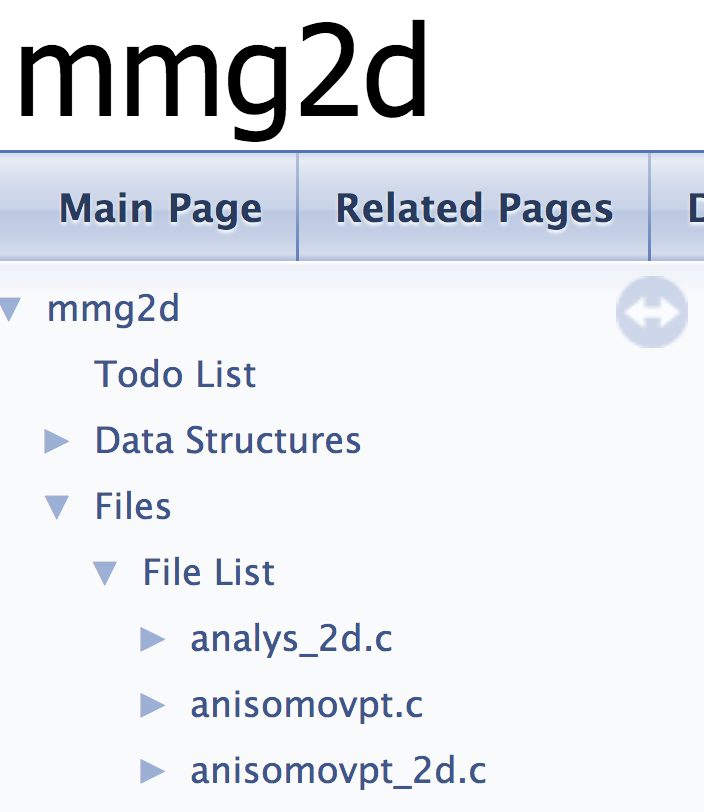
\includegraphics[width=0.3\linewidth]{Doxygen-1}
\caption{\label{dox-1}
Access to the API functions documentation in Doxygen}
\end{figure}
\item Go into the list of functions and click on the function for
  which you need informations (for example, the picture \ref{dox-2}
  shows the role and prototype of the \ttb{MMG2D\_Get\_meshSize}
    function).
\begin{figure}
\centering
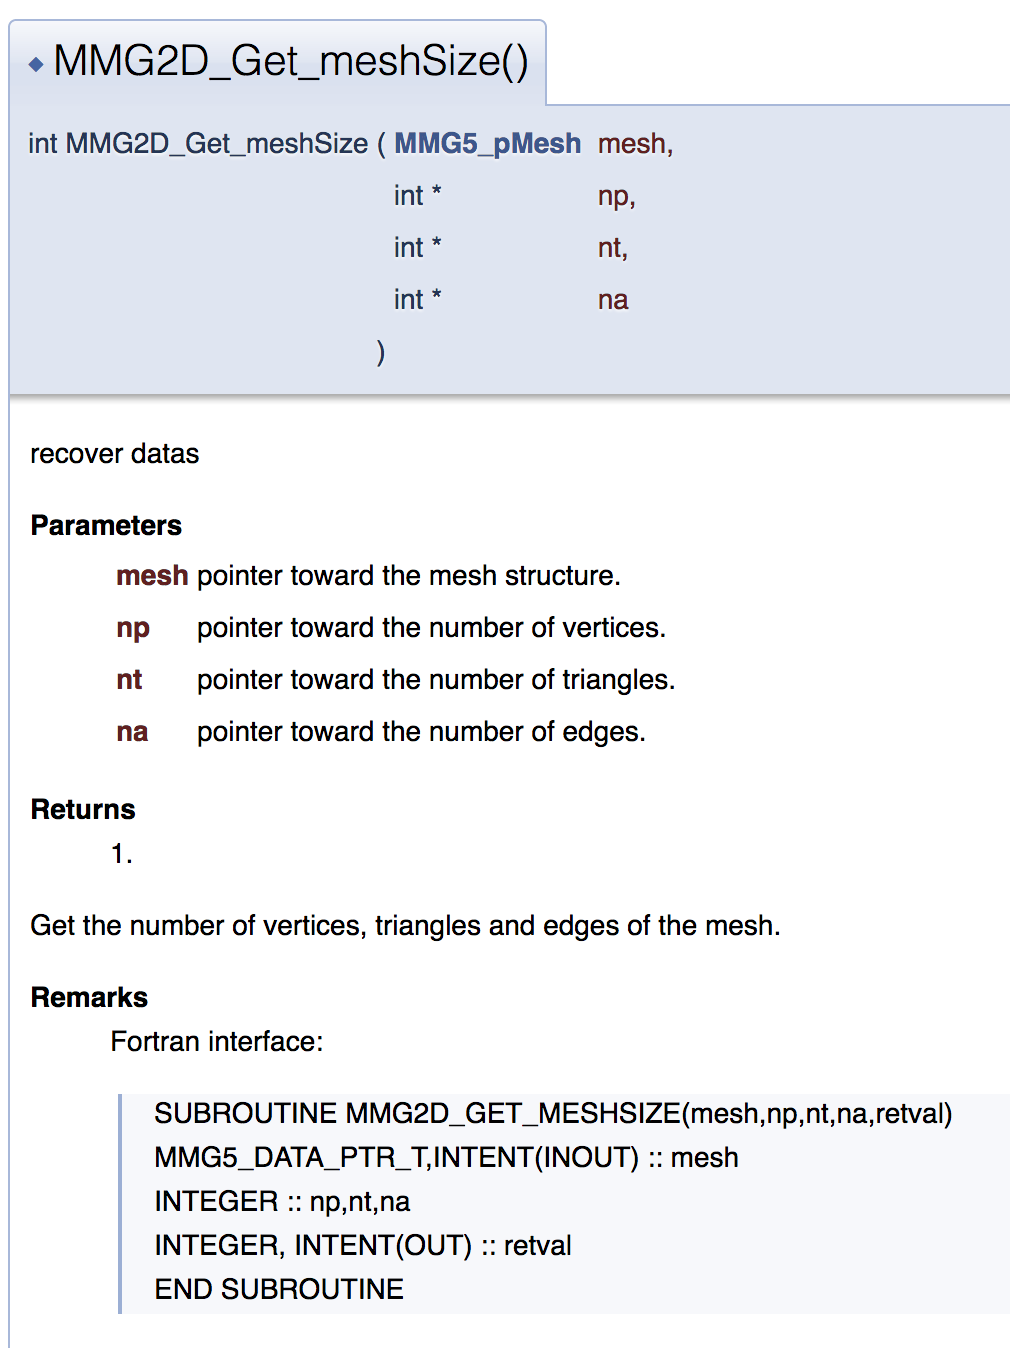
\includegraphics[width=0.5\linewidth]{Doxygen-2}
\caption{\label{dox-2}
\ttb{MMG2D\_Get\_meshSize} function in the Doxygen documentation.}
\end{figure}
\end{itemize}

A few remarks are in order for \ttb{Fortran} users:
\begin{itemize}
\item The \ttb{Fortran} prototypes are given in the \ttb{Remarks} section of
  the documentation. In general, \ttb{Fortran} arguments are the same than the \ttb{C}
  arguments with an additional integer argument (the last one) to
  store the return value of the fortran subroutine.
\item For \ttb{C} variadic function (\ttb{Init\_mesh} and \ttb{Free\_all}),
  it is not possible to provide a \ttb{Fortran} interface, thus, wrong
  arguments can be passed without error at build time.
\end{itemize}

You can open the program file and try to understand what is done.

\subsection{Build an application that calls the mmg2d library}
You can build the application with the following command:
\begin{lstlisting}[language=bash]
$ gcc firstSizeMap.c -o firstSizeMap -L $MMG_PATH/build/lib/ -lmmg2d
  -I $MMG_PATH/build/include/ -lm
\end{lstlisting}
where the \ttb{\$MMG\_PATH} variable must be replaced by your path
through the Mmg directory (\ttb{Fortran} users just need to use a \ttb{Fortran} compiler
instead of a \ttb{C} one and to replace the \ttb{firstSizeMap.c} file by the
\ttb{firstSizeMap.F90} one). Doing so creates the \ttb{firstSizeMap} application.\\

Call this application and look at its outputs.

\subsection{Size map computation}

\textcolor{red}{Je ne comprends pas... Dans quel cas te places-tu ? Quel maillage ?}
We will create a size map associated with an edge length equal to 
\begin{itemize}
\item 0.05 inside a
ball of center (0,0) and radius 3 
\item 0.2 outside this ball.
\end{itemize}
In other terms, a finer mesh is required near the nose of the naca. 

To achieve this purpose, we need to
specify to \mmg\ the size and type of the solution and
the solution value at each mesh node:
\begin{enumerate}
\item Once the mesh is stored, get its size (number of nodes,
  elements...) and create a scalar solution with the suitable size;
\item Perform a loop over the mesh nodes and get their coordinates.
\item Uncomment the call to the \ttb{scalar\_size} function and fill
  this function: given the (x,y) coordinates of a vertex, it must
  compute the wanted edge size at this vertex;
\item Set the computed size in the size map with the \ttb{Set\_scalarSol} function.\\
\end{enumerate}

 Run your program, check your initial size map (\ttb{init.mesh} file)
 and the final mesh (\ttb{firstSizeMap.mesh}).\\

%%%%%%%%%%%%%%%%%%%%%%%%%
\section{Size map computation to control the interpolation error of an analytic function over the mesh\label{error_interp}}
%%%%%%%%%%%%%%%%%%%%%%%%%

\subsection{Computation of the nodal values of a 2d analytic function}
\begin{enumerate}
\item Choose a function $f : \mathbb{R}^2 \to \mathbb{R}$, for example, 
  $$f(x,y) = \sin\left(\frac{x}{2}+\frac{y}{2}\right);$$
\item Compute its nodal values at the mesh nodes. You may start from
  the \ttb{Data/createSol.c} and \ttb{Data/createSol.F90} files and
  fill the function \ttb{f} ;
\item Build the application (the \ttb{\$MMG\_PATH} variable must be
  replaced by your path through the Mmg directory):
\begin{lstlisting}[language=bash]
$ gcc createSol.c -o createSol -L $MMG_PATH/build/lib/ -lmmg2d
  -I $MMG_PATH/build/include/ -lm
\end{lstlisting}
Doing so creates the \ttb{createSol} application.
\item This application takes 3 arguments: your inital mesh, the wanted
  maximal error of interpolation ($\epsilon$) and the type of metric
  that you want to compute: 0 for a scalar metric (in the case of isotropic adaptation), 1 for a matrix
  one (in the case of anisotropic adaptation). 
  For example, to create the anisotropic metric that prescribes
  edge lengths allowing to have a maximal error of $0.01$ over the
  \ttb{naca\_embedded.mesh} file:
\begin{lstlisting}[language=bash]
  $ ./createSol naca_embedded.mesh 0.01 1
\end{lstlisting}
This command generates 3 files:
\begin{itemize}
\item \ttb{vizuSolution.mesh} that allows to vizualize the analytic function;
\item \ttb{vizuMet.mesh} that allows to vizualize the computed metric;
\item \ttb{adaptedMesh.mesh}, the final mesh that makes even the interpolation error.
\end{itemize}
Note that at this step, the metric computation is not yet implemented
thus \ttb{vizuMet.mesh} contains uninitialized values and the
remeshing step must not been performed.
\end{enumerate}

%%%%%%%%
\subsection{Computation of a size map to control the interpolation error over the mesh}
%%%%%%%%

\textcolor{red}{Pas clair du tout... Il faut peut-\^etre expliquer un peu plus la th\'eorie derri\`ere, et donner une r\'ef\'erence...?}
The error of interpolation at a mesh node $V$, we want to compute
the matrix $M(V)$ such as:
$$
M(V) = \frac{2}{9\epsilon} \, \left | H_u(V) \right | = \frac{2}{9\epsilon} \, R
\left |\Lambda\right | R^{-1}.
$$

\subsubsection{Anisotropic size map}
You can compute the tensor metric $M(V)$ inside the \ttb{tensor\_size}
function of the \ttb{createSol.c} file. Use the \ttb{siz} array (of
size 3) to store $m_{11}$, $m_{12}$ and $m_{22}$ ($m_{21} = m_{12}$ so
it is useless to store it).\\

To achieve this, proceed as follows:

\begin{enumerate}
\item Compute $H(V)$, the Hessian of the previous analytical function
  at a node $V$. This matrix is symetric definite positive, thus, it
  is possible to store only 3 of the 4 tensor data inside a 1D array:
  $h_{11},\,h_{12},\,h_{22}$. (you can implement this
  inside the \ttb{hessian} function of the \ttb{createSol.c} file);
\item compute $\bar{H}(V) = \frac{2}{9\epsilon}H(V)$;
\item compute the eigenvectors and the absolute value of the
  eigenvalues of $\bar{H}(V)$ (you can use the given \ttb{eigenvals}
  function that computes the eigenvectors and eigenvalues of a
  symetric matrix);
\item a null eigenvalue (which physically means that we want an
  infinite edge) will create numerical issues (division by 0), thus, we
  need to truncate the maximal edge length. Truncate the maximal edge
  length by a suitable value (for example, 10. is a suitable value for
  the \ttb{naca\_embedded.mesh} mesh).
\item compute $M(V) = R \bar{\Lambda} R^{-1}$, with
  $\bar{\Lambda}$ the diagonal matrix of the truncated absolute values
  of the eigenvalues of $\bar{H}(V)$.
\end{enumerate}


Open the \ttb{vizuMet.mesh} file to vizualize your anisotropic metric field.
You can click over a node to print the ellipse associated to the prescribed metric.\\

Open the \ttb{adaptedMesh.mesh} file to see the final result.

\subsubsection{Isotropic size map}
You can implement the computation of the isotropic edge length at a
node $V$ in the \ttb{scalar\_size} function of the \ttb{createSol.c}
file:

\begin{enumerate}
\item Perform the 4 steps of the previous section;
\item Find $\bar{\lambda}$, the maximum value of the truncated absolute values
  of the eigenvalues of $\bar{H}(V)$ and compute
  $ s(V) = \frac{1}{\sqrt{\bar{\lambda}}}$.
\end{enumerate}
Run the application and check your isotropic metric
field as well as the adapted mesh.\\

A correction for the exercices in Sections \ref{size_map} and
\ref{error_interp} is available in the \ttb{Correction} folder of this repository.

%%%%%%%%%%%%%%%%%%%%%%%%%%%%%%%%%%%%%%%%%%%%%%%%%%%%%%%
\begin{thebibliography}{00}
%%%%%%%%%%%%%%%%%%%%%%%%%%%%%%%%%%%%%%%%%%%%%%%%%%%%%%%

\bibitem{Dapogny2014}
{\sc C. Dapogny, C. Dobrzynski and P. Frey}, {\em Three-dimensional adaptive domain remeshing,
  implicit domain meshing, and applications to free and moving boundary
  problems}, Journal of Computational Physics. 2014;\hspace{0pt}262:358--378.

\bibitem{dobFrey}{\sc C. Dobrzynski and P. Frey}, {\em Anisotropic Delaunay Mesh Adaptation for Unsteady Simulations}, Proc. 17th Int. Meshing Roundtable, Pittsburgh, (2008).

\end{thebibliography}


\end{document}
